\documentclass[11pt,a4paper]{article}

% ==========================================================
% PACKAGES
% ==========================================================

\usepackage[margin=2.4cm]{geometry}
\usepackage{graphicx}
\usepackage{booktabs}
\usepackage{amsmath}
\usepackage{amssymb}
\usepackage{siunitx}
\usepackage{float}
\usepackage{hyperref}
\usepackage{xcolor}
\usepackage{array}
\usepackage{enumitem}

\hypersetup{
    colorlinks=true,
    linkcolor=blue,
    urlcolor=blue
}

\newcommand{\graphplaceholder}[2]{
    \begin{figure}[H]
        \centering
        \fbox{
            \begin{minipage}[c][5.2cm][c]{0.82\textwidth}
                \centering
                \textbf{GRAPH PLACEHOLDER}\\[0.4cm]
                #1
            \end{minipage}
        }
        \caption{#2}
    \end{figure}
}

% ==========================================================
% DOCUMENT
% ==========================================================

\title{
    \textbf{GaN Quantum Dot Detection and Analysis}\\
    \large Project Overview and Current Methodology
}

\author{Poline}
\date{\today}

\begin{document}

\maketitle
\tableofcontents
\newpage


% ==========================================================
\section{Project Overview}
% ==========================================================

The purpose of this project is to develop and evaluate an automated pipeline for the detection and quantitative characterisation of semiconductor quantum dots (QDs) from atomic force microscopy (AFM) images.

Analysis pipeline is as follows:

\begin{enumerate}[itemsep=2pt]
    \item convert the original AFM data into a convenient numerical representation;
    \item remove scan tilt, line artefacts and slowly varying background structure;
    \item identify candidate quantum dots;
    \item estimate physical QD parameters such as position, height, radius, area and FWHM;
    \item compare automatically obtained results against manually curated ground truth;
    \item compare classical image-processing algorithms with machine-learning approaches.
    \item optimise the final selected algorithm for the best F1 score.
\end{enumerate}


% ==========================================================
\section{Repository Structure}
% ==========================================================

The project is divided into a small number of sections.

\begin{table}[H]
\centering
\small
\begin{tabular}{p{0.31\textwidth} p{0.61\textwidth}}
\toprule
\textbf{File / directory} & \textbf{Purpose} \\
\midrule

\texttt{Data-Conversion/}
&
Conversion of raw AFM data into NumPy arrays used by the analysis code. It also stores all unlabelled AFM data.
\[
\mathrm{.spm}
\rightarrow
\mathrm{.gwy}
\rightarrow
\mathrm{.npy}.
\]
\\[2mm]

\texttt{Image-Preprocessing/}
&
Artefact removal so that it is easier to detect QDs.
\\[2mm]

\texttt{Ground-Truth/}
&
Stores all labelled datasets used for model training, model itself and height/ FWHM manual data from Xin. Contains an app created to label QDs (heavily inspired by Cobi's)
\\[2mm]

\texttt{detection\_algorithms.py}
&
Implementation of the classical QD detection algorithms using a common output structure.
\\[2mm]

\texttt{detection\_errors.py}
&
Functions for quantitative comparison of predicted and ground-truth detections.
\\[2mm]

\texttt{QD-gui.py}
&
Interactive interface for viewing and analysing QDs in AFM scans with an option to select multiple detection algorithms, different thresholds and kernels for Top Hat.
\\[2mm]

\texttt{method-COMPARISON.ipynb}
&
Notebook used for comparison of different QD detection approaches.
\\[2mm]

\texttt{npy-data-QD-DETECTION.ipynb}
&
Experimental notebook for applying QD detection methods to NumPy AFM data. Used to summarise what I learned about image processing and demonstrate why certain algorithms have been chosen.
\\[2mm]

\texttt{npy-data-QD-ANALYSIS.ipynb}
&
Notebook for subsequent analysis of detected quantum dots. Contains a comparison of physical characteristic of QDs growing on GaN and InGaN layers.
\\[2mm]

\texttt{npy-data-TRANSFORMS.ipynb}
&
Notebook used for testing and visualising transformations applied to AFM images.
\\

\bottomrule
\end{tabular}
\caption{High-level organisation of the repository.}
\end{table}


% ==========================================================
\section{AFM Data Conversion}
% ==========================================================

\subsection{\texttt{Data-Conversion/spm-to-gwy.py}}

The original microscope measurements are stored in SPM files. The first conversion stage handles these microscope-specific files and converts them into Gwyddion-compatible data.

Using an intermediate Gwyddion representation is useful because Gwyddion understands the structure and metadata of common AFM formats and provides a convenient bridge between the proprietary microscope format and ordinary numerical arrays.


\subsection{\texttt{Data-Conversion/gwy-to-npy.py}}

The second conversion stage reads Gwyddion files and searches recursively for two-dimensional data fields corresponding to image channels.

Each detected two-dimensional channel is converted to a NumPy array and saved as a separate \texttt{.npy} file.

The resulting arrays are the principal numerical input used throughout the rest of the project.


% ==========================================================
\section{Image Preprocessing}
% ==========================================================

AFM scans contain structure unrelated to the quantum dots themselves. Examples include sample tilt, scanner-induced line offsets, stripes and slowly varying background curvature.
Instead of having to open Gwyddion everytime to preprocess the image, the same can be done in either of the GUIs.

Direct application of a detection algorithm to the raw image can therefore produce incorrect QD positions and measurements.

The preprocessing code is divided into two files in order to not mix usual and more advanced processes for dealing with artefacts and show ideas development in a more orderly way.


% ----------------------------------------------------------
\subsection{\texttt{basic\_data\_preprocessing.py}}
% ----------------------------------------------------------

This file contains the main general-purpose AFM preprocessing operations.

\subsubsection{Robust normalisation}

Images can be rescaled using a robust estimate based on the median and median absolute deviation rather than the ordinary mean and standard deviation.

This reduces influence of unusually high QD peaks when estimating image typical scale.


\subsubsection{Global plane removal}

Large-scale sample tilt is modelled as

\[
z(x,y)=ax+by+c.
\]

The fitted plane is subtracted from the AFM image. The plane fit uses iterative outlier rejection so that strong foreground features have less influence on the estimated background.


\subsubsection{Scan-line flattening}

AFM images are acquired line-by-line. Individual scan lines may contain their own offsets or gradients. Each line can therefore be fitted independently using a low-order polynomial, which is then removed.

\[
p(x)=\sum_{k=0}^{d}a_kx^k,
\]

Robust fitting is again used to reduce the effect of quantum-dot peaks on the fitted background.


\subsubsection{Scan-line alignment}

Even after flattening, neighbouring scan lines may exhibit abrupt vertical offsets. The median value of each row is estimated and compared with a smoothed trend. Rapid changes in row height can then be removed while retaining slower physical variation.


\subsubsection{Combined preprocessing pipeline}

The standard preprocessing function currently combines the principal operations in sequence:

\[
\text{raw image}
\rightarrow
\text{plane removal}
\rightarrow
\text{line flattening}
\rightarrow
\text{row alignment}.
\]

Though, when labelling the data I only used line fitting so that less data is modified (though, correlation between raw image and 'destriped image' ame out to be 99 percent).

\begin{figure}[H]
    \centering
    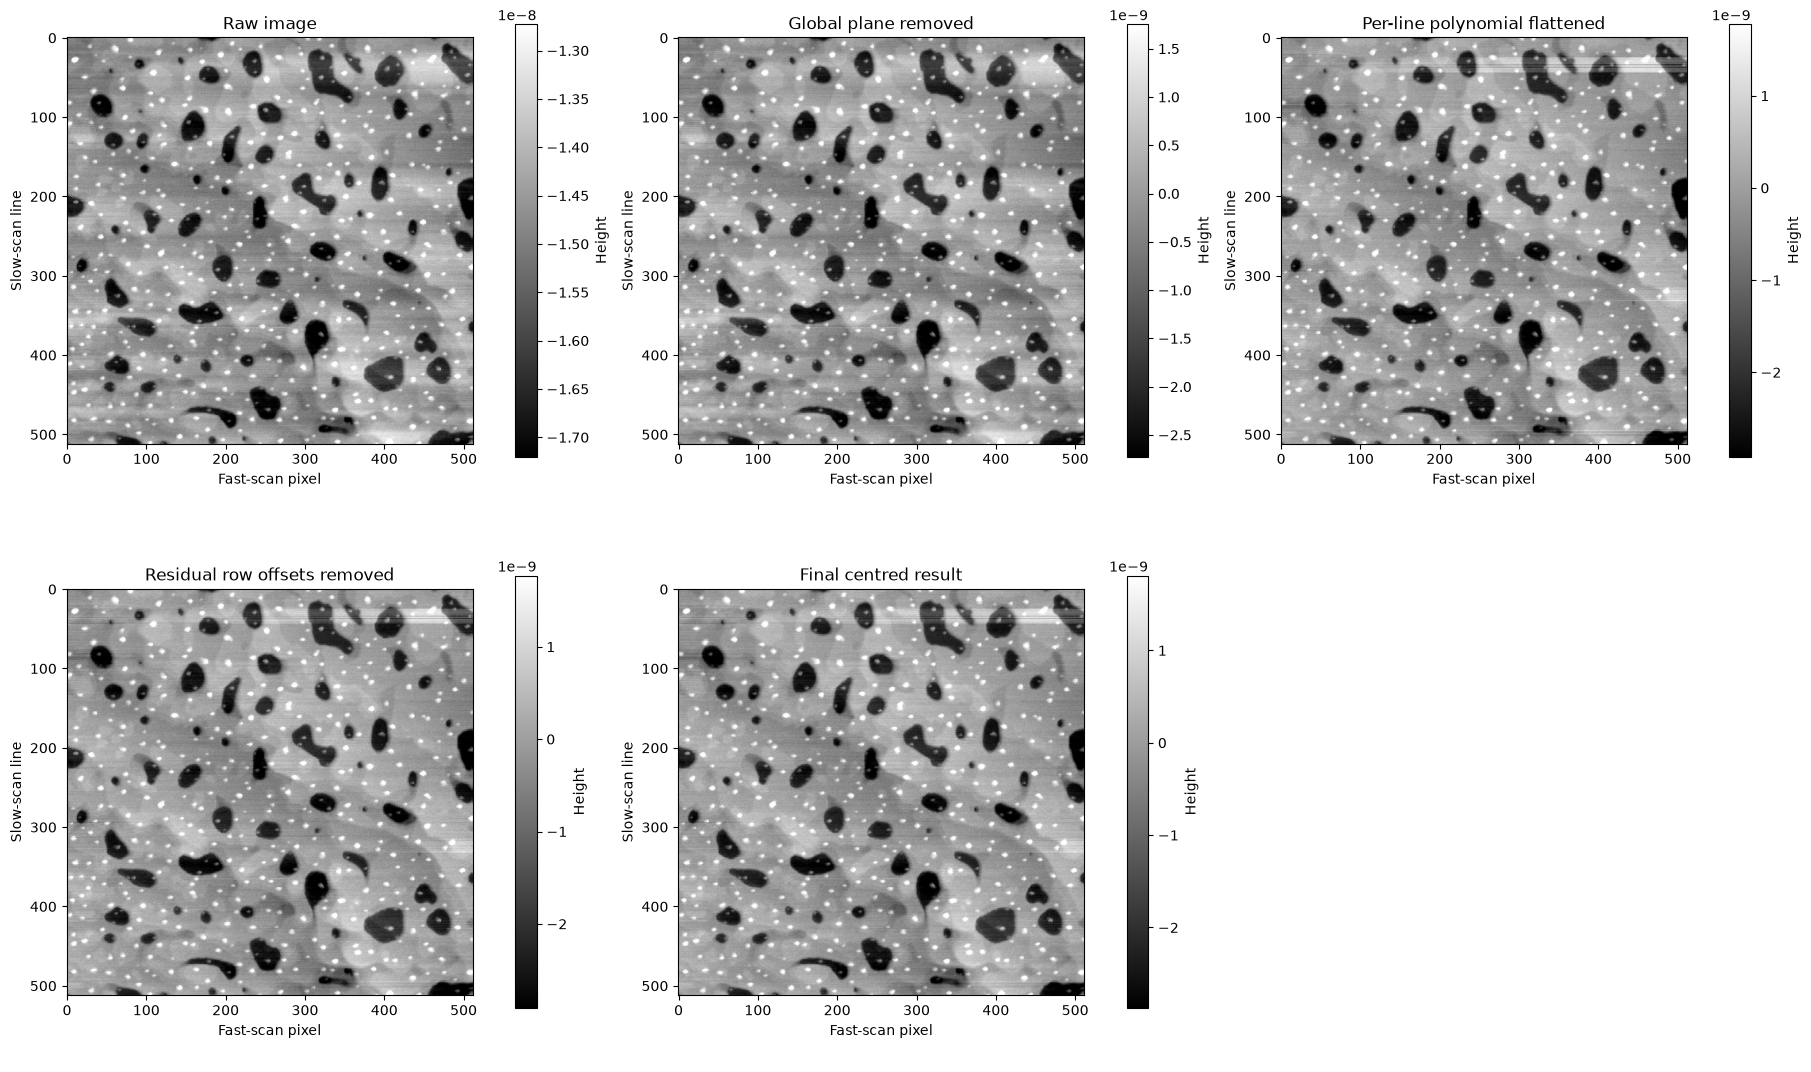
\includegraphics[width=0.85\textwidth]{References/basicpreprocessing.png}
    \caption{Applying basic preprocessing techniques.}
    \label{fig:basicpreprocessing.png}
\end{figure}


% ----------------------------------------------------------
\subsection{\texttt{foreground\_preprocessing.py}}
% ----------------------------------------------------------

A limitation of ordinary background fitting is that quantum dots themselves may influence the fitted surface.

If a polynomial is fitted to every pixel, large QD peaks can pull the estimated background upward. Subtracting this background may then remove part of the physical QD height that is actually of interest.

The foreground-aware method addresses this problem iteratively:

\begin{enumerate}[itemsep=2pt]
    \item fit an initial polynomial background;
    \item calculate the residual image;
    \item identify sufficiently large positive residuals as probable foreground;
    \item dilate the foreground mask to exclude QD edges;
    \item refit the polynomial using only probable background pixels;
    \item repeat the procedure;
    \item subtract the final fitted background.
\end{enumerate}

This is intended to provide a stronger background-removal method for AFM images containing convex objects such as quantum dots.


\begin{figure}[H]
    \centering
    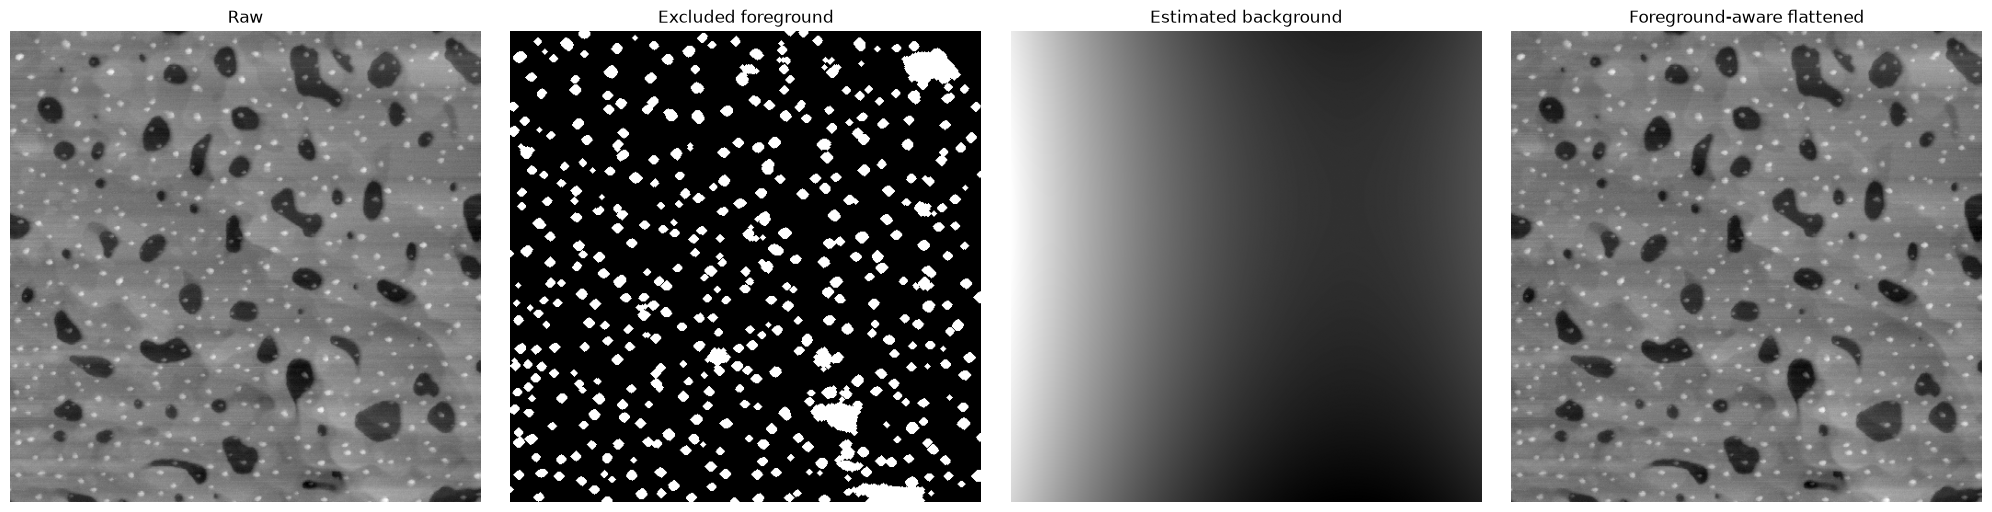
\includegraphics[width=0.85\textwidth]{References/imagepreprocessing_foreground.png}
    \caption{Foreground-aware preprocessing of the AFM image.}
    \label{fig:foreground-preprocessing}
\end{figure}


% ==========================================================
\section{Ground-Truth Construction}
% ==========================================================

The \texttt{Ground-Truth/} directory contains the manually curated reference data used to evaluate the algorithms and train the machine-learning model.


% ----------------------------------------------------------
\subsection{\texttt{NPY-Ground-Truth/}}
% ----------------------------------------------------------

This directory contains paired AFM images and binary masks.

For a scan,

\begin{itemize}[itemsep=2pt]
    \item \texttt{channel\_00\_\_\_0\_data.npy} contains the AFM height image;
    \item \texttt{channel\_00\_\_\_0\_data\_mask.npy} contains the corresponding ground-truth QD mask;
    \item feature CSV files can store measured properties of individual dots.
\end{itemize}

The binary masks are used both for algorithm evaluation and supervised machine-learning training.


% ----------------------------------------------------------
\subsection{\texttt{QD-gui-npy-TRAINING-SETS.py}}
% ----------------------------------------------------------

The ground-truth GUI provides an interactive method for constructing and correcting QD masks.

Initial QD candidates are generated automatically, after which detections can be manually corrected.

The editor supports operations such as removal of false-positive detections, ddition of false-negative QDs, local QD-height measurement, FWHM measurement, export of corrected masks, export of QD feature information to CSV files.

This allows the training and evaluation data to be manually inspected instead of assuming that an automatically generated segmentation is correct.


\begin{figure}[H]
    \centering
    \includegraphics[width=0.85\textwidth]References/training_gui.png
    \caption{Labelling App GUI.}
    \label{fig:training_gui.png}
\end{figure}


% ----------------------------------------------------------
\subsection{\texttt{initiation-tests.py}}
% ----------------------------------------------------------

This is a small diagnostic script. It checks that image and mask files are loaded correctly and reports properties such as image dimensions, data types, number of QD pixels and number of connected QD regions.

Its purpose is primarily dataset verification rather than QD detection itself.


% ==========================================================
\section{Classical Quantum-Dot Detection}
% ==========================================================

\subsection{Noise Reduction}

Before applying feature-detection algorithms, noise in the AFM image should be reduced. Two principal approaches considered in this project are \textbf{Gaussian smoothing} and \textbf{anisotropic diffusion}.
Gaussian smoothing applies the same type of smoothing everywhere, whereas anisotropic diffusion adapts the amount of smoothing according to the local image gradient.

\subsubsection{Gaussian Smoothing}

Gaussian smoothing replaces each pixel by a weighted average of neighbouring pixels. The weighting kernel is a two-dimensional Gaussian,

\[
G(x,y;\sigma)
=
\frac{1}{2\pi\sigma^2}
\exp\left(
-\frac{x^2+y^2}{2\sigma^2}
\right),
\]

and the smoothed image is obtained by convolution,

\[
I_{\sigma}(x,y)
=
G(x,y;\sigma) * I(x,y),
\]

where \(I(x,y)\) is the original image and \(*\) denotes convolution.

Pixels close to the centre of the Gaussian receive a larger weight than pixels further away. The parameter \(\sigma\) determines the spatial scale over which averaging occurs.

A small value of \(\sigma\) produces weak smoothing and preserves fine features, whereas a larger value suppresses more high-frequency variation.

Gaussian smoothing is therefore a \textbf{linear and isotropic} filtering operation. This makes the method simple and computationally efficient, but it also means that genuine QD boundaries may be blurred together with noise.

\subsubsection{Anisotropic Diffusion}

Anisotropic diffusion instead treats image smoothing as a diffusion process whose strength depends on the local image gradient.

The image evolves according to

\[
\frac{\partial I}{\partial t}
=
\nabla \cdot
\left(
c(|\nabla I|)\nabla I
\right),
\]

where

\[
\nabla I
\]

is the local image gradient and \(c(|\nabla I|)\) is a diffusion coefficient.

If \(c\) were constant, this equation would reduce to ordinary diffusion, which is closely related to Gaussian smoothing. In anisotropic diffusion, however, \(c\) decreases when the image gradient becomes large.

A commonly used Perona--Malik diffusion coefficient is

\[
c(|\nabla I|)
=
\exp\left[
-\left(
\frac{|\nabla I|}{\kappa}
\right)^2
\right],
\]

or alternatively,

\[
c(|\nabla I|)
=
\frac{1}{
1+\left(
\frac{|\nabla I|}{\kappa}
\right)^2
}.
\]

The parameter \(\kappa\) determines which gradients are interpreted as significant boundaries.

In approximately uniform regions,

\[
|\nabla I| \ll \kappa,
\]

so

\[
c(|\nabla I|) \approx 1,
\]

and diffusion proceeds strongly, smoothing noise.

At a strong boundary,

\[
|\nabla I| \gg \kappa,
\]

the diffusion coefficient approaches zero, so smoothing across that boundary is suppressed. Consequently, anisotropic diffusion can remove noise from relatively flat regions while preserving sharp QD boundaries.

\subsection{QD detection algorithms}

\begin{center}
\texttt{detection\_algorithms.py}.
\end{center}

\begin{figure}[H]
    \centering
    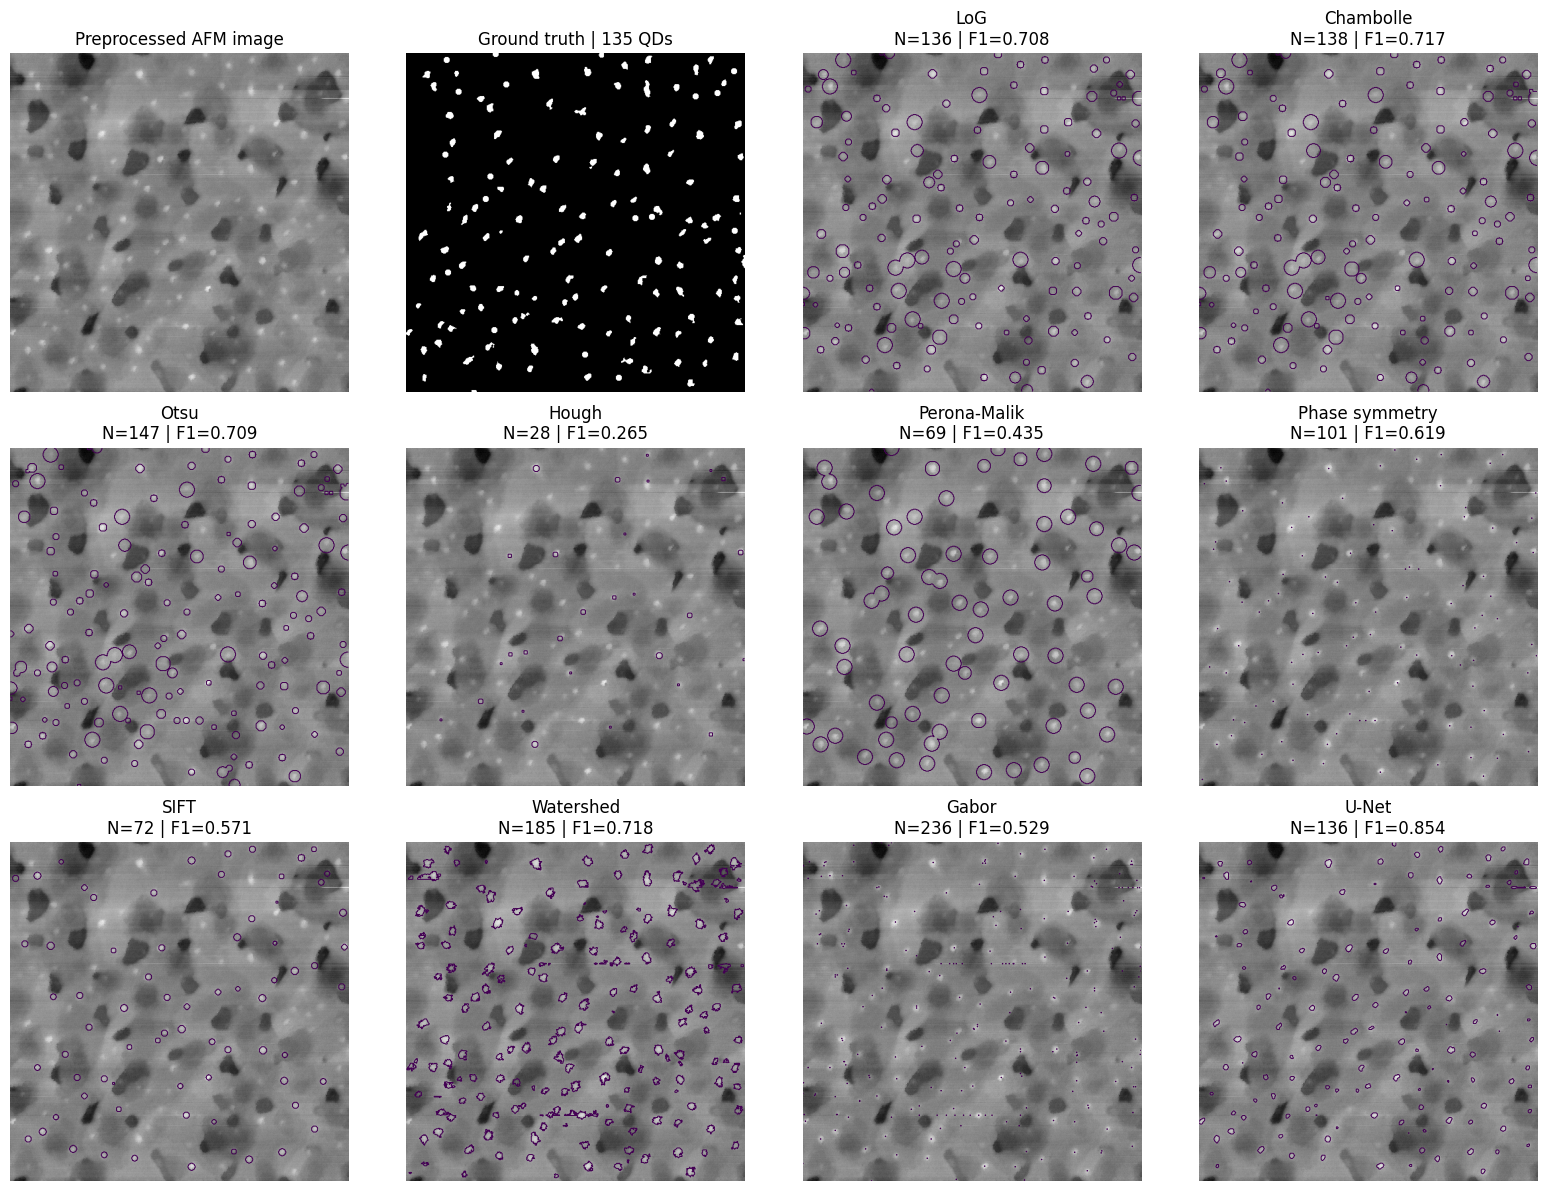
\includegraphics[width=1.1\textwidth]{References/detection_comparison.png}
    \caption{Detection algorithms vs Ground Truth.}
\end{figure}


A common output representation is used. Typical outputs include a binary detection mask, QD centre coordinates, measured local heights, estimated radii, estimated areas. Results are retained before and after application of the physical minimum-height criterion.


\subsubsection{Laplacian of Gaussian (LoG) Detection}

Useful for identifying approximately blob-like structures such as quantum dots.

The method combines two operations:

\begin{enumerate}
    \item smoothing the image with a Gaussian filter to suppress high-frequency noise (but I added a function to use anisotropic diffusion instead);
    \item applying the Laplacian operator, which measures the second spatial derivative of the smoothed image. This detects a feature based on gradient changes.
\end{enumerate}

For a bright approximately circular object on a darker background, the LoG response becomes large when the scale of the Gaussian is comparable to the size of the object.

Therefore, instead of using only one value of \(\sigma\), the image can be filtered over a range of scales to detect different features. A candidate blob is detected when the magnitude of the LoG response forms a local maximum in both spatial position and scale.
Thus LoG detection also provides an approximate characteristic size.

\begin{figure}[H]
    \centering
    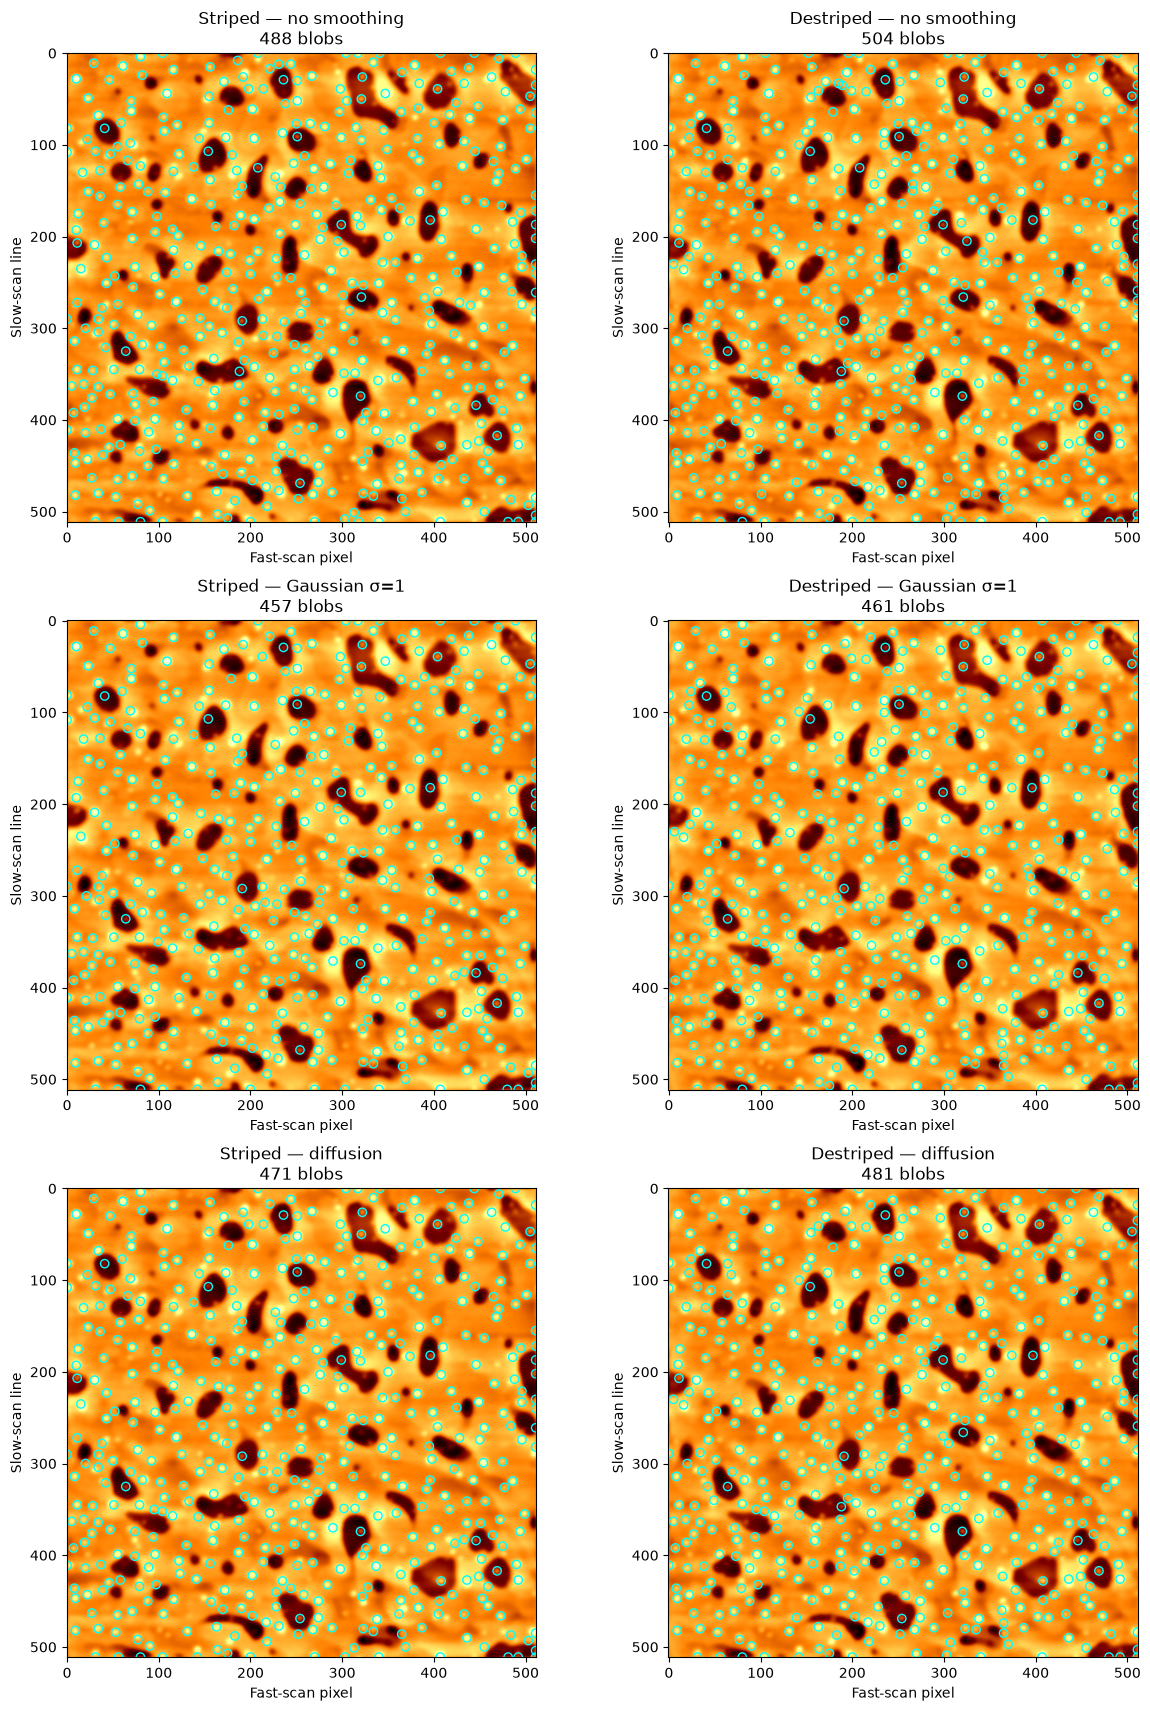
\includegraphics[width=0.8\textwidth]{References/gaussiananisotropicnosmoothing.png}
    \caption{LoG and different smoothing techniques.}
\end{figure}


\subsubsection{Otsu Thresholding}

It aims for the maximum separation between classes of objects. Thresholding converts a continuous-valued image or detector response into a binary mask by assigning pixels either to background or foreground:

\[
M(x,y)=
\begin{cases}
1, & I(x,y) > T,\\
0, & I(x,y) \leq T,
\end{cases}
\]

where \(T\) is the chosen threshold.

\begin{figure}[H]
    \centering
    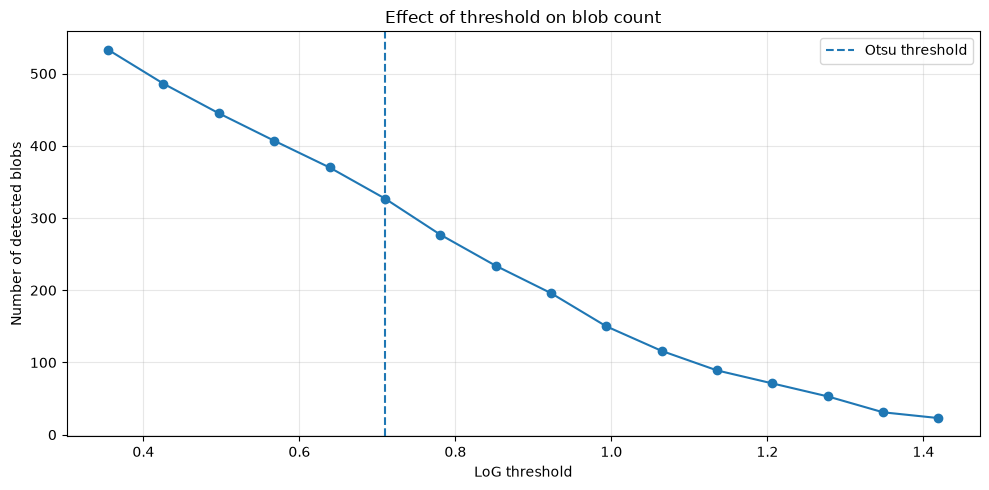
\includegraphics[width=0.8\textwidth]{References/otsuthreshold.png}
    \caption{Impact of Otsu threshold on QD detection.}
\end{figure}

Otsu's method chooses the threshold automatically from the intensity distribution of the image. It assumes that the histogram can be approximately separated into two classes: a lower-valued background class and a higher-valued foreground class.

For every possible threshold \(T\), the pixels are divided into

\[
C_0 = \{I \leq T\},
\qquad
C_1 = \{I > T\}.
\]

For these two classes, Otsu's method calculates their probabilities

\[
\omega_0(T), \qquad \omega_1(T),
\]

and their mean intensities

\[
\mu_0(T), \qquad \mu_1(T).
\]

It then selects the threshold that maximises the separation between the two classes. This is quantified by the between-class variance,

\[
\sigma_B^2(T)
=
\omega_0(T)\omega_1(T)
\left[
\mu_0(T)-\mu_1(T)
\right]^2.
\]

The selected threshold is therefore

\[
T^*
=
\arg\max_T \sigma_B^2(T).
\]

In other words, Otsu's method searches for the threshold that makes the background and foreground groups as distinct as possible.

There is also Otsu detection for multiple object classes. But Multi-Otsu does not know what a GaN, substrate, or QD is.It only separates the histogram into three groups.
\begin{enumerate}
    \item 0 = GaN 
    \item = InGaN
    \item = bright QD
\end{enumerate}

\begin{figure}[H]
    \centering
    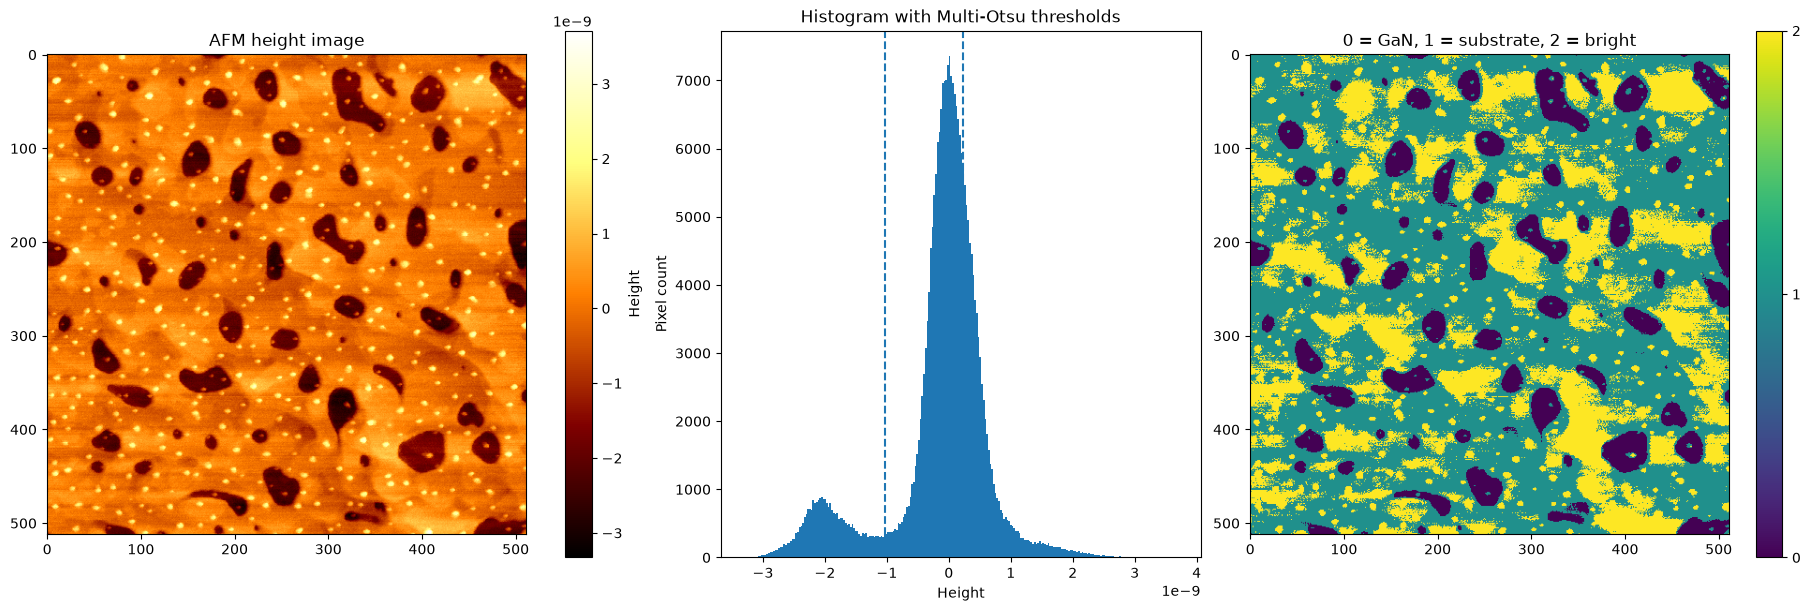
\includegraphics[width=0.8\textwidth]{References/multiotsu.png}
    \caption{Multi-Otsu.}
    \label{fig:multi-otsu.png}
\end{figure}

Since this didn't seem to be working, I applied other thresholding techniques that delped me separate QDs within and outside the GaN layer (see more choices in ANALYSIS notebook).

\begin{figure}[H]
    \centering
    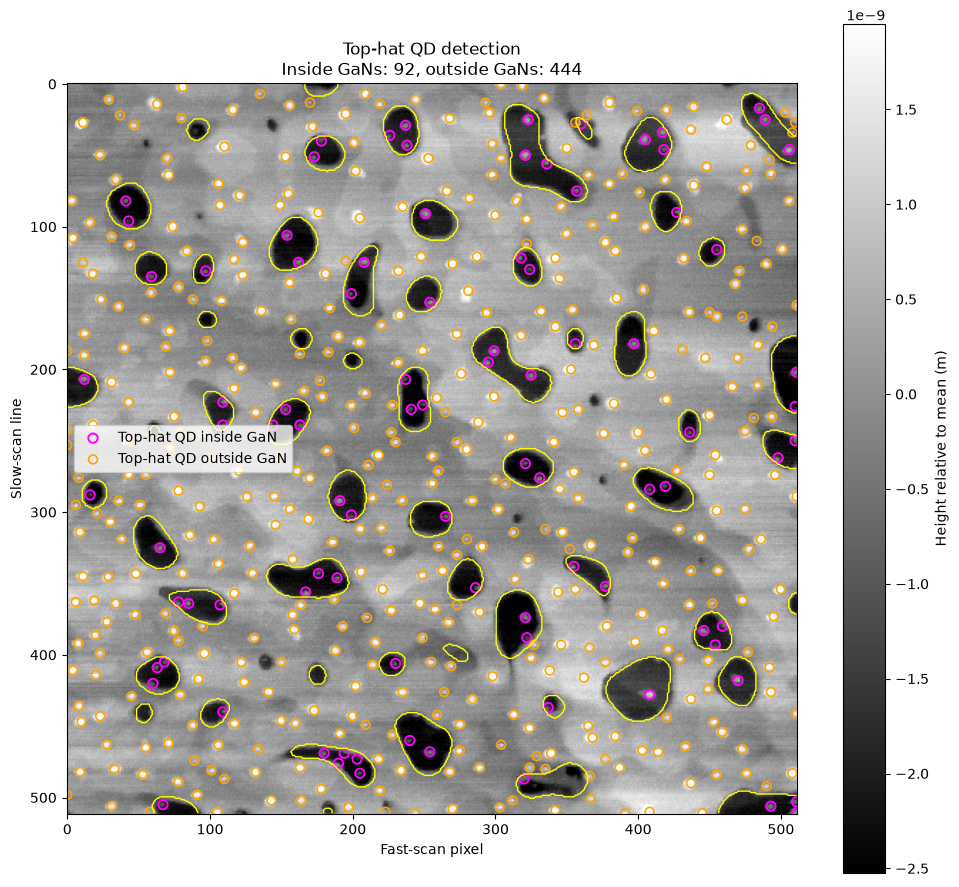
\includegraphics[width=0.8\textwidth]{References/qdganingan.png}
    \caption{Other thresholding techniques.}
\end{figure}


\subsubsection{Hough transform}

Circular Hough transforms search explicitly for approximately circular structures over a selected range of radii. Whether an object is a QD or not is decided by the majority votes. 

This introduces stronger geometric assumptions than LoG detection. However, I have also tried using the General Hough Transform to be able to detect all the different QD shapes and find out other potential geometric characteristics.

\begin{figure}[H]
    \centering
    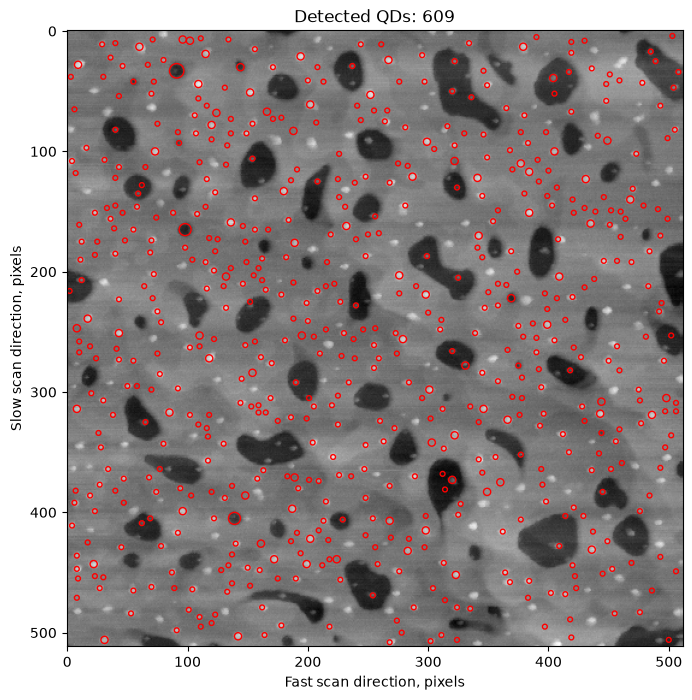
\includegraphics[width=0.48\textwidth]{References/HT.png}
    \hfill
    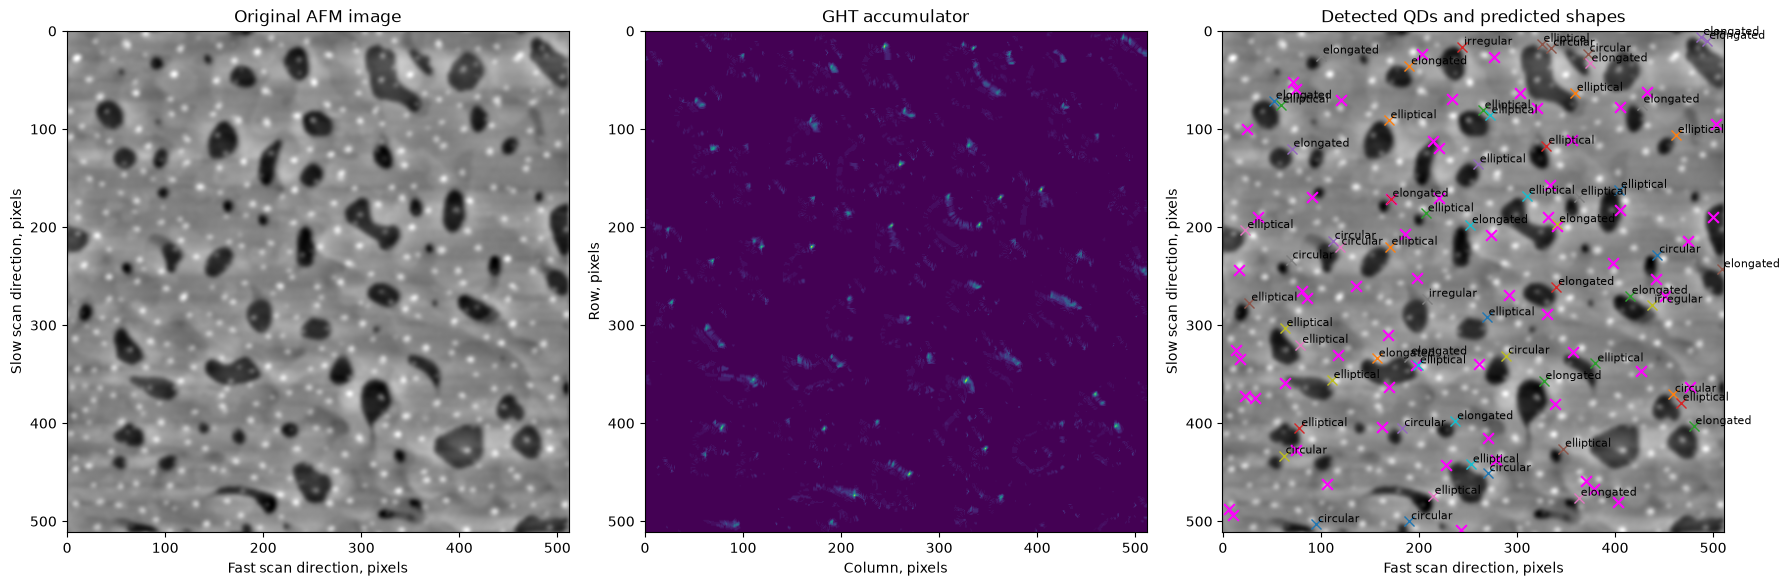
\includegraphics[width=0.48\textwidth]{References/GHT.png}
    \caption{Comparing HT and GHT.}
\end{figure}

While this wasn't the best detection algorithm, it was still helpful for identifying geometric properties of an individual dot: 
\begin{figure}[H]
    \centering
    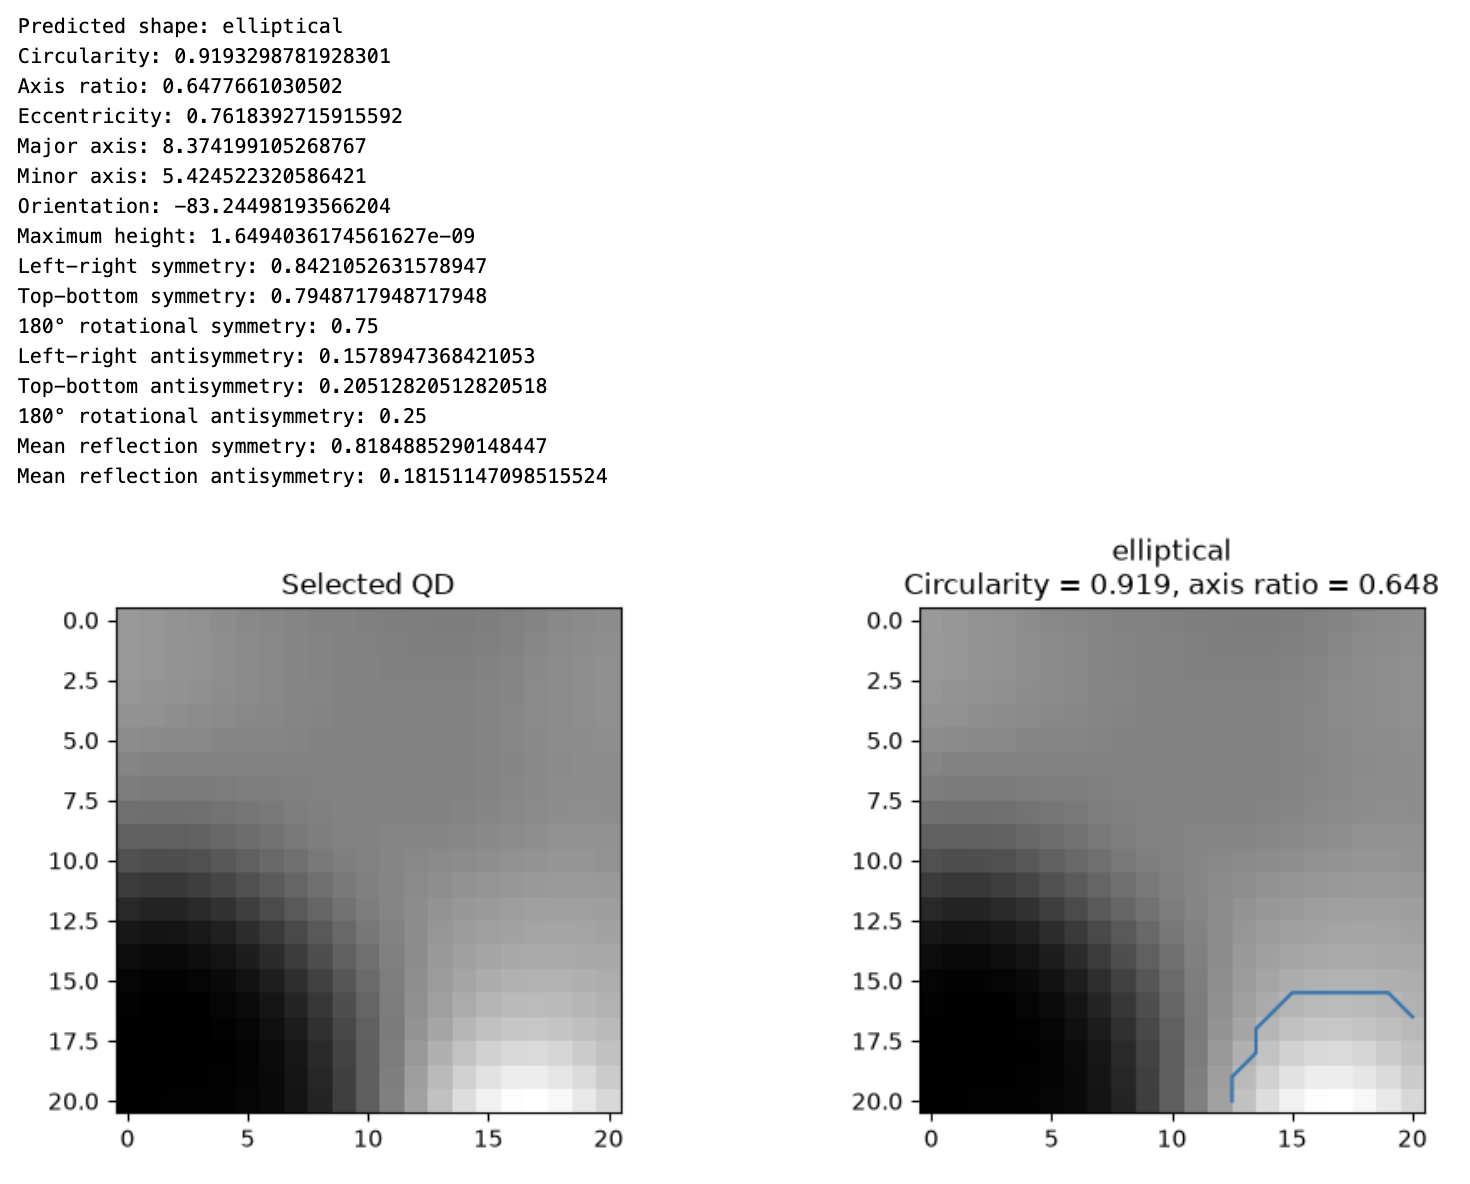
\includegraphics[width=0.48\textwidth]{References/individualQD.png}
    \hfill
    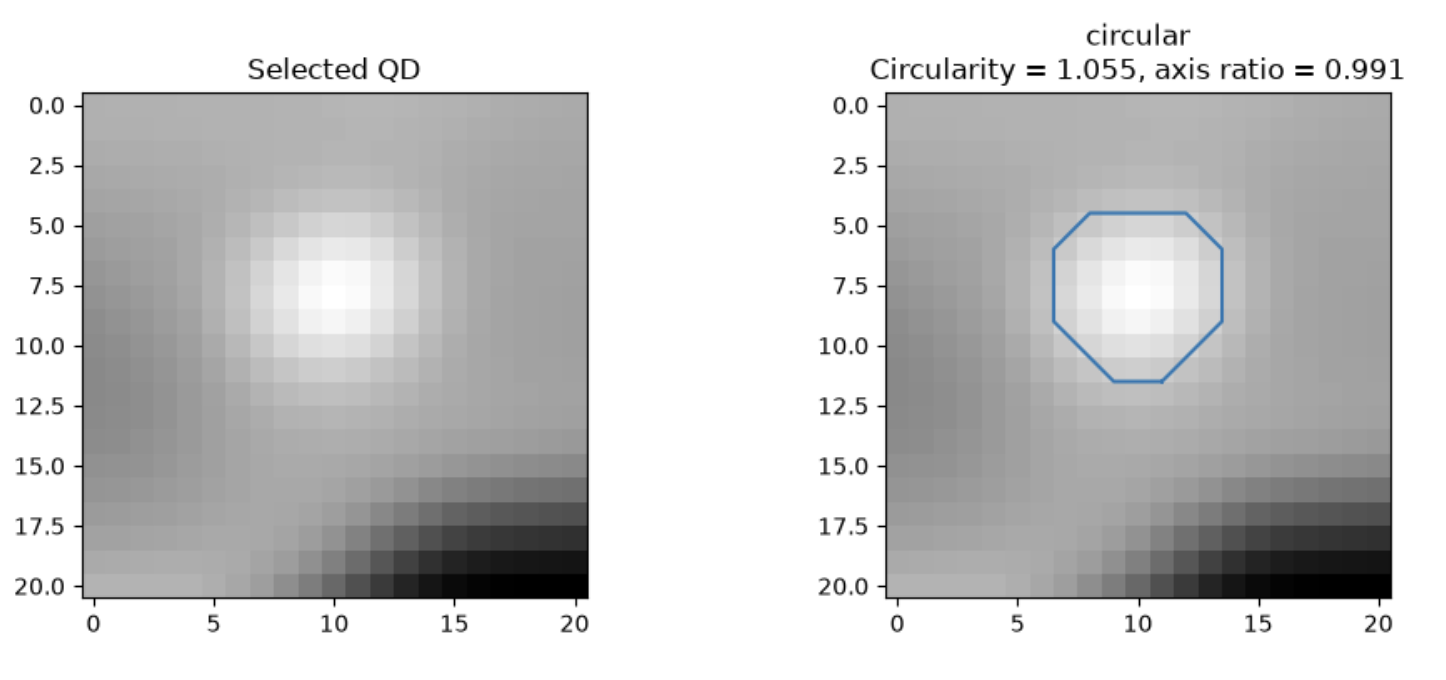
\includegraphics[width=0.48\textwidth]{References/individualcircleqd.png}
    \caption{Comparing HT and GHT.}
\end{figure}

\subsubsection{Phase symmetry}

Phase-based detection attempts to identify locally symmetric image structures. Because it depends on local phase information rather than absolute intensity alone, it provides a qualitatively different approach to identifying QD-like objects.

It utilsies the fact that an edge or a line appears where several waves of different sizes reach a peack, trough, or 0 at the same position. And this can be determined by convolving a set of wavelets with an image and calculating the differnce between the average filter responses. These wavelets are called Gabor wavelets.

\begin{figure}[H]
    \centering
    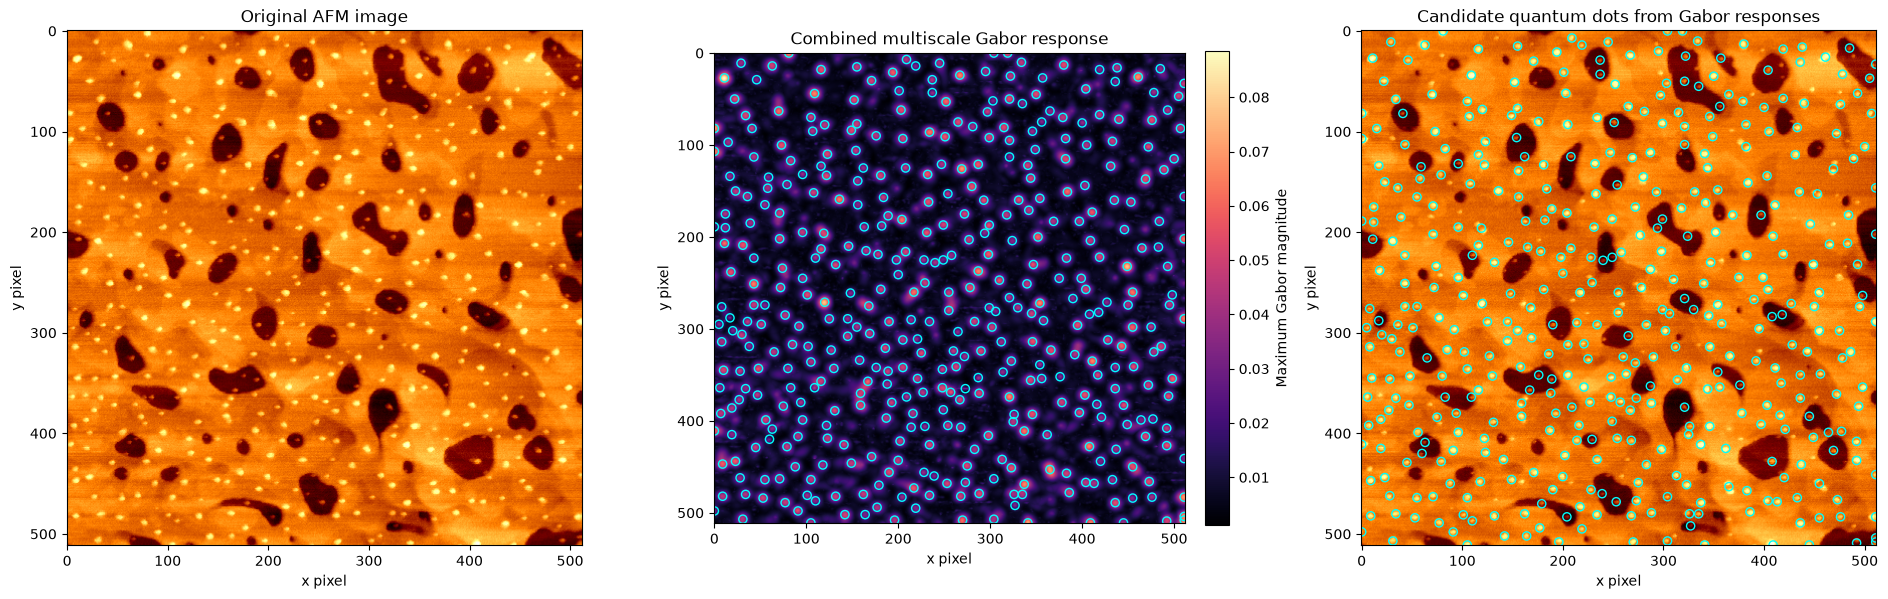
\includegraphics[width=0.8\textwidth]{References/gaborwavelets.png}
    \caption{Gabor wavelets.}
\end{figure}

\begin{figure}[H]
    \centering
    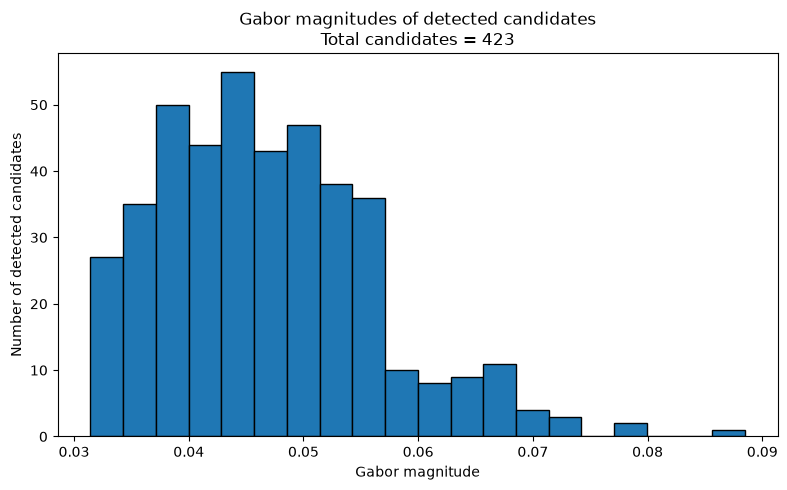
\includegraphics[width=0.48\textwidth]{References/gaborresponses.png}
    \hfill
    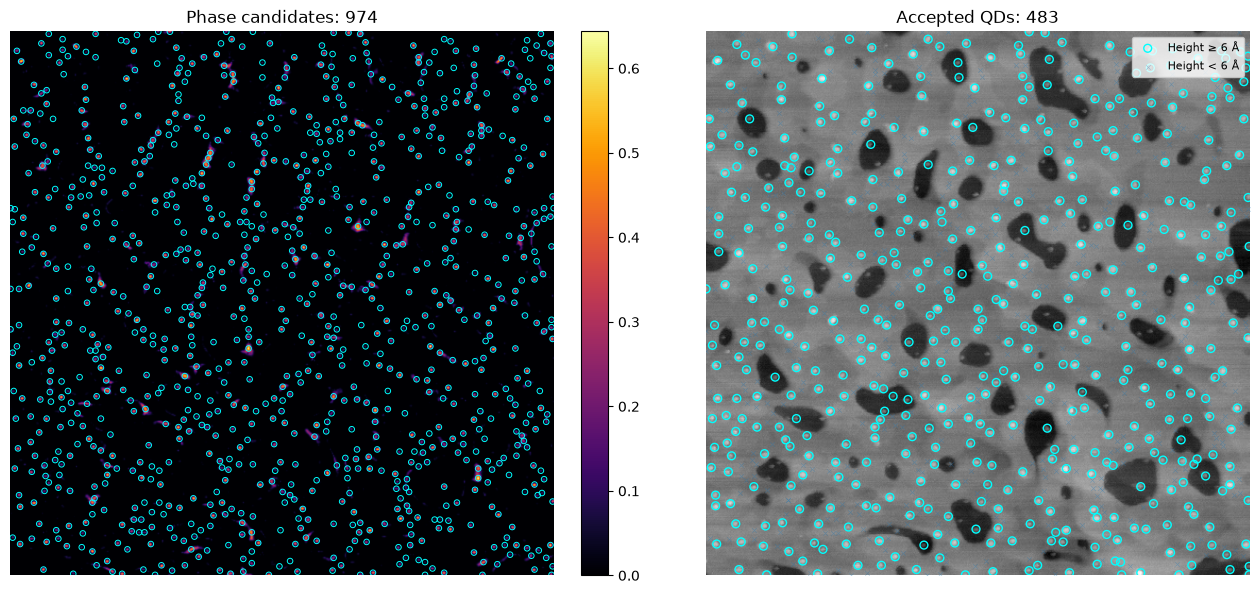
\includegraphics[width=0.48\textwidth]{References/phasecongrouency.png}
    \caption{Gabor responses and Phase congruency.}
\end{figure}

\subsubsection{SIFT}

This finds distinctive points in an image and describes the local pattern around each point so that the same feature can be recognised in another range.

I wasn't expecting a lot from this method, as QDs seemed to all be having a bit different shapes and tehrefore it may be hard to be using different QDs' features to recognise others.

\begin{figure}[H]
    \centering
    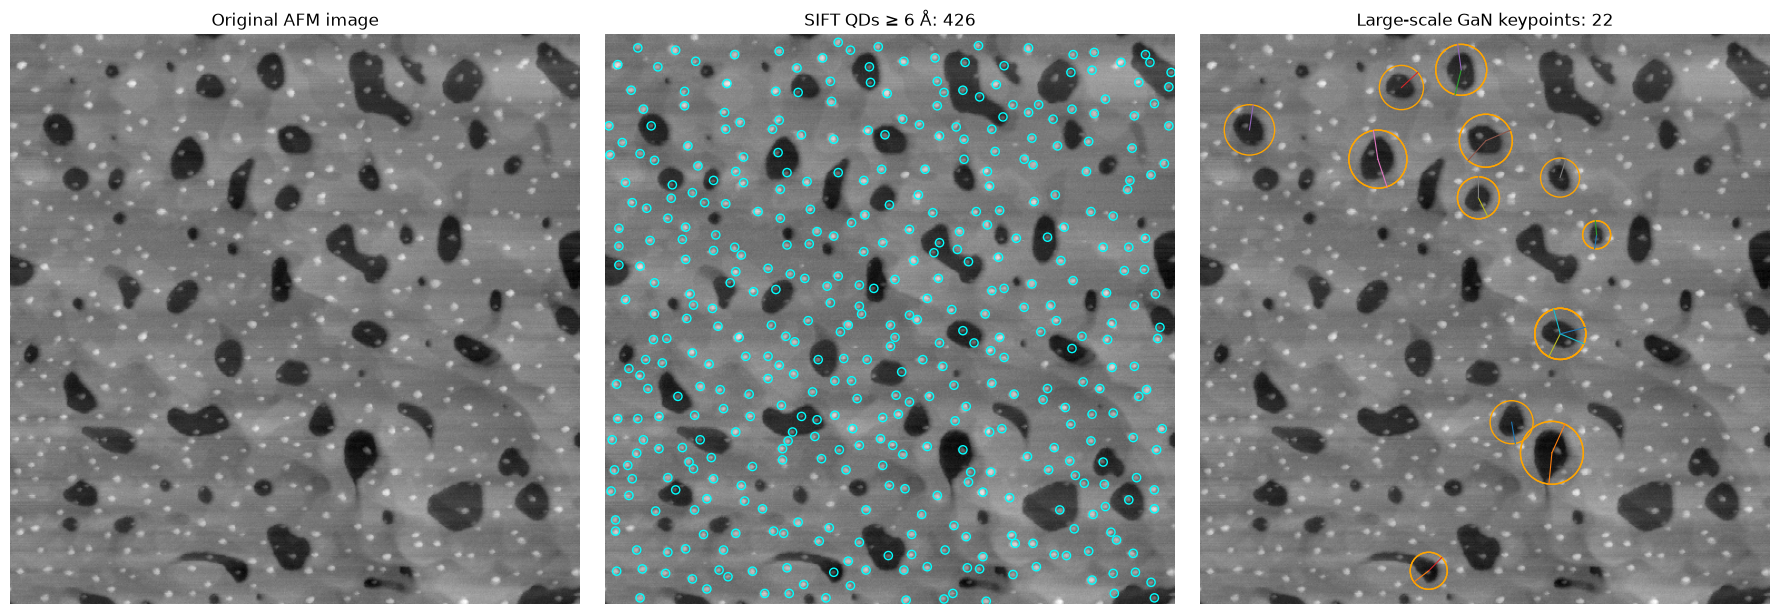
\includegraphics[width=0.8\textwidth]{References/sift.png}
    \caption{SIFT for small and large scales.}
\end{figure}

SIFT examines the image across multiple spatial scales rather than analysing only one filtered version of the image.

A scale-space representation is formed by convolving the image \(I(x,y)\) with Gaussian kernels of increasing standard deviation \(\sigma\):

\[
L(x,y,\sigma)
=
G(x,y,\sigma) * I(x,y),
\]

where increasing \(\sigma\) removes progressively finer image detail.

SIFT then subtracts nearby Gaussian-blurred images to form the Difference of Gaussians (DoG):

\[
D(x,y,\sigma)
=
L(x,y,k\sigma)
-
L(x,y,\sigma).
\]

The Difference of Gaussians approximately behaves like a scale-normalised Laplacian of Gaussian:

\[
D(x,y,\sigma)
\approx
(k-1)\sigma^2 \nabla^2 L(x,y,\sigma).
\]

Therefore, the DoG produces a strong response around blob-like structures whose characteristic size matches the current scale \(\sigma\).

Candidate keypoints are identified from strong local extrema of the DoG response across both image position and scale. If the DoG response is too small,

\[
|D(x,y,\sigma)| < T,
\]

the candidate is likely to correspond to noise or a weak image feature and can be rejected.

SIFT also assigns an orientation to each retained keypoint using the local image gradient. The orientation may be written as

\[
\theta(x,y)
=
\operatorname{atan2}
\left(
\frac{\partial L}{\partial y},
\frac{\partial L}{\partial x}
\right),
\]

which describes the predominant direction of local intensity change around the feature.

The combination of scale-space analysis, DoG extrema and local gradient information allows SIFT to detect local structures over a range of characteristic sizes rather than relying on a single fixed spatial scale.

\subsection{Active Contours}

Active contours refine an approximate QD boundary by starting from an initial region and iteratively deforming it to better match the image.

Two approaches are used in this project:

\subsubsection{Morphological Geodesic Active Contours (MGAC)}

MGAC is an \textbf{edge-based} method. It evolves the contour towards regions with a strong image gradient, which are assumed to correspond to QD boundaries.

An edge indicator can be written as

\[
g(I)=\frac{1}{1+\alpha |\nabla I|^2}.
\]

In smooth regions, \(g(I)\) is large and the contour can continue moving. Near a strong edge, \(g(I)\) becomes small and the contour tends to stop.

Thus,

\[
\boxed{\text{MGAC finds the QD boundary using gradients.}}
\]

\subsubsection{Chan--Vese}

Chan--Vese is instead a \textbf{region-based} method and does not require a sharp edge.

It moves the contour so that the pixels inside and outside it are as different as possible while remaining relatively uniform within each region:

\[
E =
\lambda_1 \int_{\mathrm{inside}} (I-c_1)^2\,dx\,dy
+
\lambda_2 \int_{\mathrm{outside}} (I-c_2)^2\,dx\,dy,
\]

where \(c_1\) and \(c_2\) are the mean intensities inside and outside the contour.

Thus,

\[
\boxed{\text{Chan--Vese finds the boundary using differences between regions.}}
\]

For QD detection, MGAC is most useful when the dot has a clear boundary gradient, whereas Chan--Vese can still work when the transition from the QD to the surrounding background is gradual.

\begin{figure}[H]
    \centering
    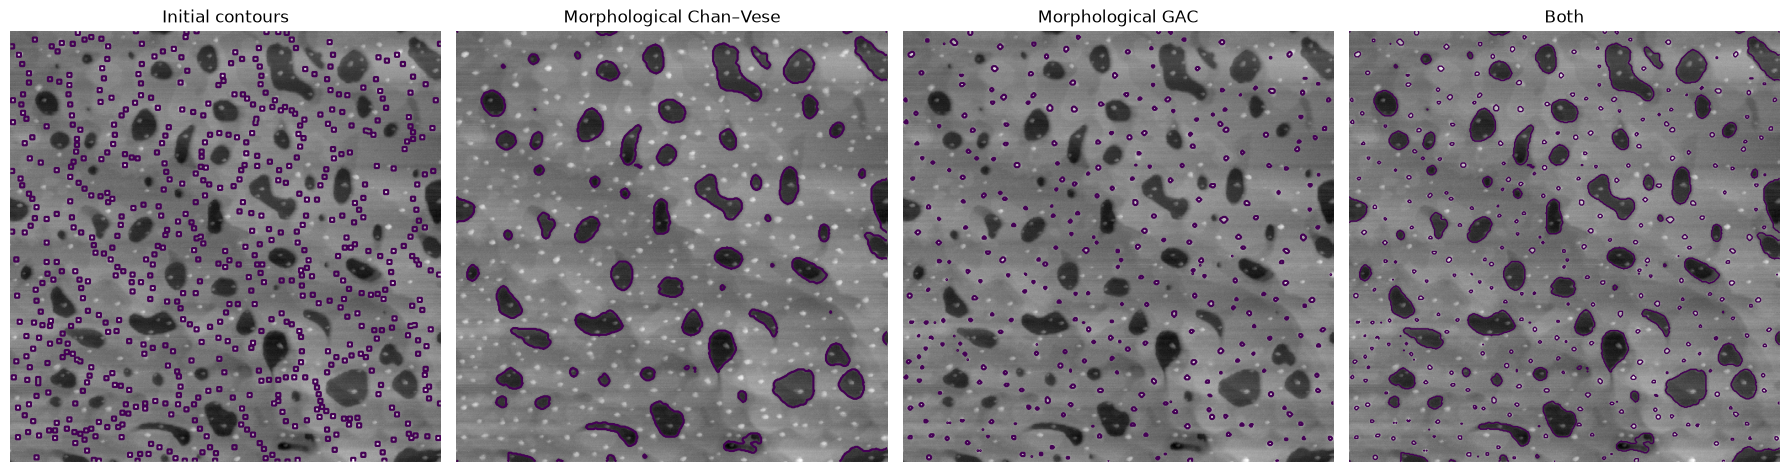
\includegraphics[width=0.8\textwidth]{References/activecontours.png}
    \caption{Comparing Active Contour Methods.}
\end{figure}


\subsection{Watershed}

The watershed implementation first enhances small bright structures using a white top-hat transformation.

After thresholding, a distance transform is calculated and local maxima are used as markers.

Watershed segmentation then separates neighbouring candidate regions.


% ==========================================================
\section{Physical QD Acceptance Criterion}
% ==========================================================

Detection based only on image shape can identify small fluctuations that are not physically meaningful QDs.

For this reason, candidate detections can be subjected to a minimum local-height requirement.

The current criterion is

\[
h_{\mathrm{QD}} \geq 6\,\AA.
\]

Local QD height is measured relative to a surrounding estimate of the local background rather than relative to one global image level.


% ==========================================================
\section{Detection Evaluation}
% ==========================================================

Evaluation utilities are primarily contained in

\begin{center}
\texttt{detection\_errors.py}
\end{center}

and

\begin{center}
\texttt{Ground-Truth/feature\_evaluation.py}.
\end{center}

The project evaluates detection at both the pixel and object levels.


% ----------------------------------------------------------
\subsection{Pixel-level metrics}
% ----------------------------------------------------------

For a predicted binary mask and ground-truth mask, standard segmentation measures include precision, recall, F1 score, Dice coefficient and intersection over union.

The Dice coefficient is

\[
D =
\frac{2|P\cap T|}
{|P|+|T|},
\]

where \(P\) is the predicted QD mask and \(T\) is the true mask.

The intersection over union is

\[
\mathrm{IoU}
=
\frac{|P\cap T|}
{|P\cup T|}.
\]


% ----------------------------------------------------------
\subsection{Object-level metrics}
% ----------------------------------------------------------

Pixel agreement does not completely describe QD detection performance.

The detected QD centres are therefore also compared with true QD centres using a spatial matching tolerance.

This provides

\begin{itemize}[itemsep=2pt]
    \item true positives;
    \item false positives;
    \item false negatives;
    \item object precision;
    \item object recall;
    \item object F1 score.
\end{itemize}

\begin{figure}[H]
    \centering
    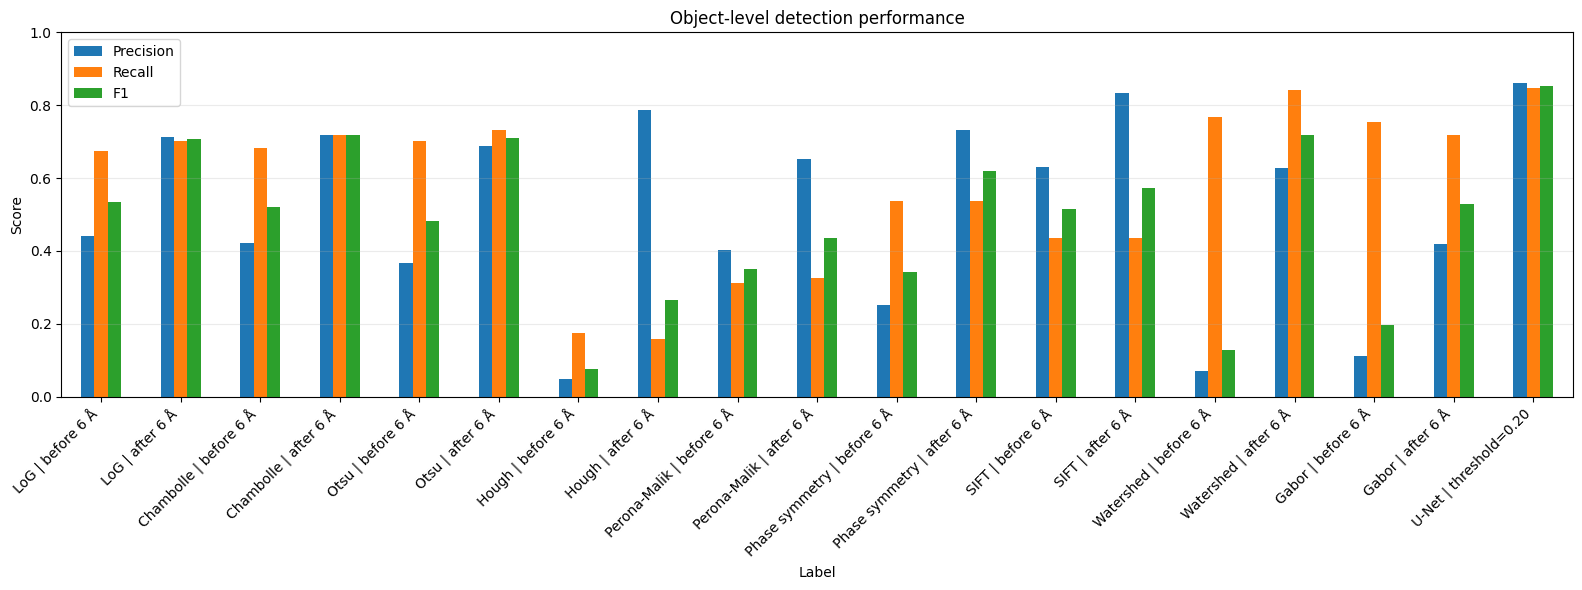
\includegraphics[width=1.0\textwidth]{References/objectlevelperformance.png}
    \caption{Foreground-aware preprocessing of the AFM image.}
    \label{fig:objectlevelperformance.png}
\end{figure}


% ----------------------------------------------------------
\subsection{Localisation and parameter errors}
% ----------------------------------------------------------

Matched QDs can additionally be compared in terms of localisation and measured physical parameters.

For example, for height,

\[
e_{h,i}
=
h_{i,\mathrm{measured}}
-
h_{i,\mathrm{true}}.
\]

The mean absolute error is

\[
\mathrm{MAE}
=
\frac{1}{N}
\sum_{i=1}^{N}
|e_i|,
\]

while the root-mean-square error is

\[
\mathrm{RMSE}
=
\sqrt{
\frac{1}{N}
\sum_{i=1}^{N}
e_i^2
}.
\]


\begin{figure}[H]
    \centering
    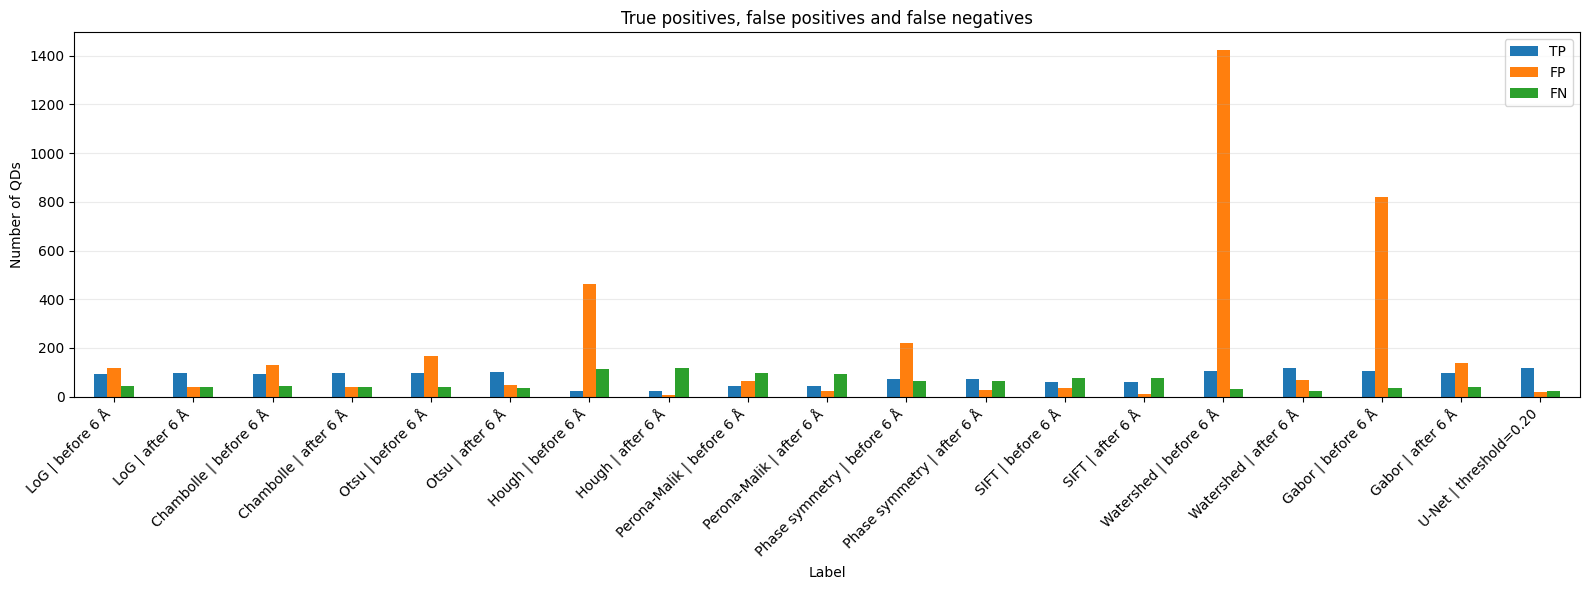
\includegraphics[width=1.0\textwidth]{References/tpfpfn.png}
    \caption{Foreground-aware preprocessing of the AFM image.}
    \label{fig:tpfpfn.png}
\end{figure}


% ==========================================================
\section{Machine-Learning Approach}
% ==========================================================

The repository also contains a supervised image-segmentation approach based on a U-Net-like convolutional neural network.


% ----------------------------------------------------------
\subsection{\texttt{Ground-Truth/model.py}}
% ----------------------------------------------------------

The model-training script loads the paired AFM scans and ground-truth masks, applies the same preprocessing pipeline used elsewhere in the project, and robustly normalises the images.

The scans are divided into training and held-out test data.

Images are subdivided into

\[
128\times128
\]

patches for training.

The implemented network contains an encoder, a bottleneck and a decoder with skip connections.

Convolutional blocks extract increasingly abstract image features while the decoder reconstructs a pixelwise QD probability map.

The final layer uses a sigmoid activation so that each output pixel lies between zero and one.


\subsection{Loss function}

Training combines binary cross-entropy with a Dice-based loss.

This is useful because QD masks are sparse: most AFM pixels belong to the background rather than to a QD.


% ----------------------------------------------------------
\subsection{\texttt{Ground-Truth/model\_prediction.py}}
% ----------------------------------------------------------

The saved network is evaluated on an unseen scan using the same preprocessing used during training.

The full image is divided into patches, each patch is passed through the network, and the predicted patches are assembled into a complete probability map.

A probability threshold is subsequently applied to obtain a binary QD mask.


\begin{figure}[H]
    \centering
    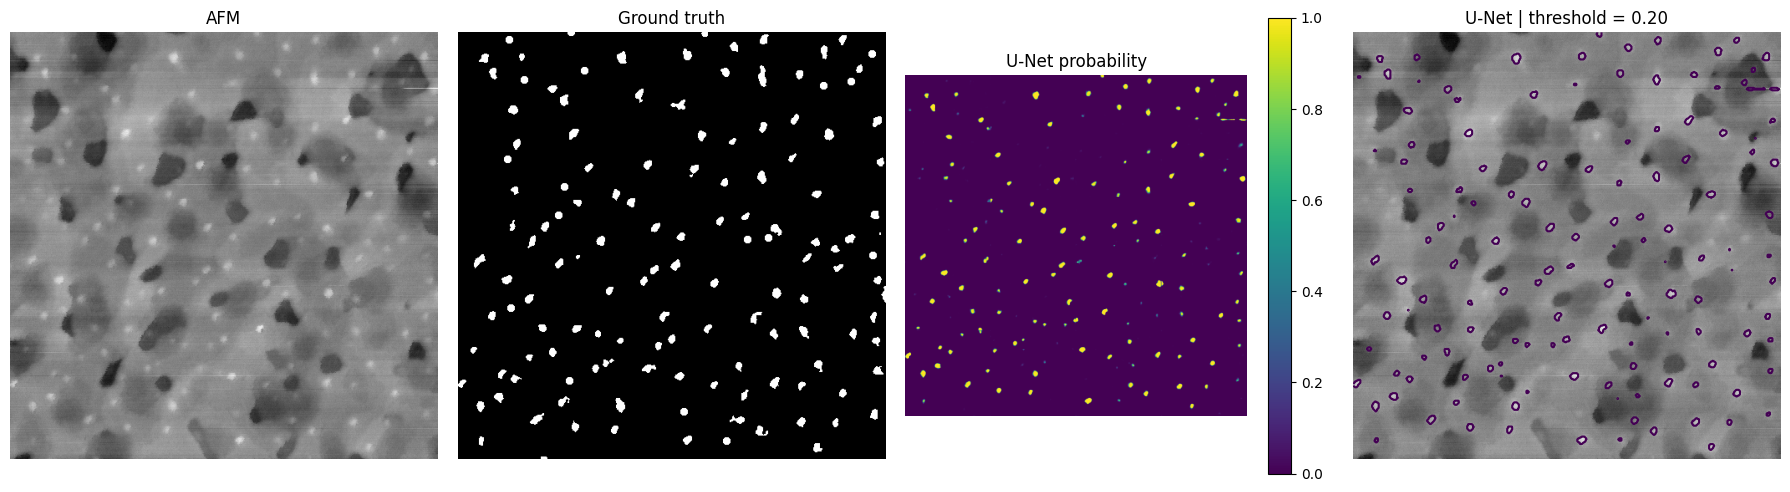
\includegraphics[width=1.0\textwidth]{References/modelperformance.png}
    \caption{Foreground-aware preprocessing of the AFM image.}
    \label{fig:modelperformance.png}
\end{figure}

\begin{figure}[H]
    \centering
    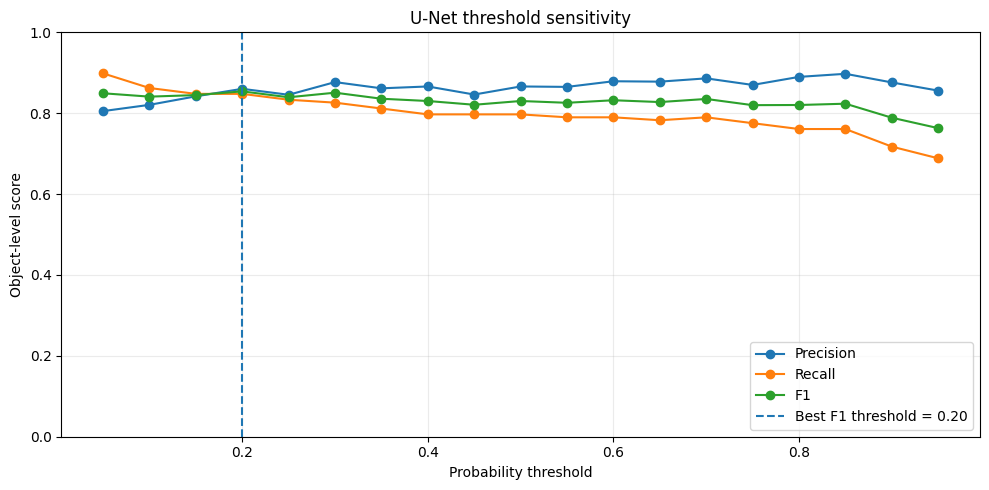
\includegraphics[width=1.0\textwidth]{References/unetsensitivity.png}
    \caption{Foreground-aware preprocessing of the AFM image.}
    \label{fig:unetsensitivity.png}
\end{figure}


% ==========================================================
\section{Height and FWHM Validation}
% ==========================================================

The directory

\begin{center}
\texttt{Ground-Truth/Height-HWFM/}
\end{center}

contains manually measured QD height and FWHM values for selected samples.

These measurements are used to determine whether the automated parameter-estimation procedure reproduces manually measured physical QD dimensions.

At present this directory contains reference CSV data for several sample conditions, the Python error-analysis script, a human-readable Excel comparison table and generated error figures.

For each matched QD,

\[
e_h
=
h_{\mathrm{automatic}}
-
h_{\mathrm{manual}}
\]

and

\[
e_{\mathrm{FWHM}}
=
\mathrm{FWHM}_{\mathrm{automatic}}
-
\mathrm{FWHM}_{\mathrm{manual}}.
\]

The resulting error distribution is important in addition to the MAE and RMSE.

A distribution centred away from zero indicates systematic bias, while a broad distribution centred near zero indicates low bias but poor precision.


\begin{figure}[H]
    \centering
    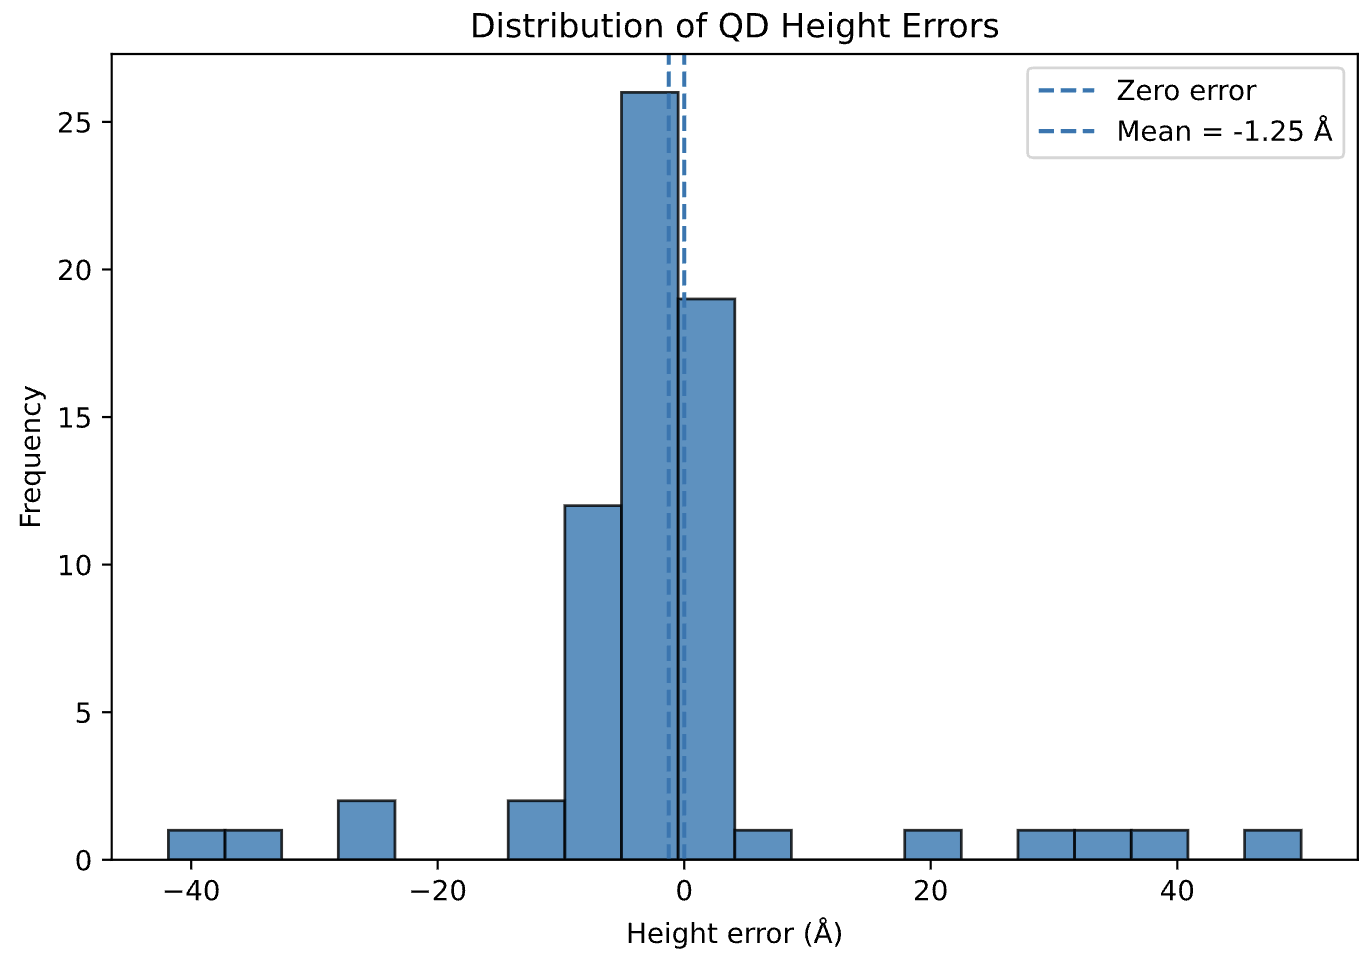
\includegraphics[width=1.0\textwidth]{References/height_error.png}
    \caption{Foreground-aware preprocessing of the AFM image.}
    \label{fig:height_error.png}
\end{figure}


% ==========================================================
\section{Analysis Notebooks}
% ==========================================================

Several notebooks are retained for interactive investigation.

\subsection{\texttt{npy-data-TRANSFORMS.ipynb}}

Used for visualising and experimenting with transformations and preprocessing applied to NumPy AFM data.

\subsection{\texttt{npy-data-QD-DETECTION.ipynb}}

Used for interactive testing of QD detection methods and detector parameters.

\subsection{\texttt{npy-data-QD-ANALYSIS.ipynb}}

Used for subsequent analysis of detected QDs and their measured properties.

\subsection{\texttt{method-comparison.ipynb}}

Provides a convenient environment for comparing the behaviour and performance of different detection methods on the same data.


% ==========================================================
\section{Graphical User Interface}
% ==========================================================

The top-level \texttt{QD-gui.py} provides an interactive interface around the analysis pipeline.

The GUI is intended to make the processing results directly inspectable rather than requiring every operation to be performed through a notebook or command-line script.

This is particularly useful for checking individual QD detections, reviewing physical measurements and understanding failure cases.



% ==========================================================
\section{Current Project Architecture}
% ==========================================================

The code can therefore be viewed as five connected layers:

\begin{enumerate}[itemsep=4pt]

    \item \textbf{Data layer}

    Raw AFM measurements are converted into two-dimensional NumPy height arrays.

    \item \textbf{Preprocessing layer}

    Large-scale background and scanner artefacts are removed while attempting to preserve physical QD morphology.

    \item \textbf{Detection layer}

    Multiple classical algorithms and a neural network estimate which structures correspond to QDs.

    \item \textbf{Physical measurement layer}

    Detected QDs are assigned positions and morphological parameters such as local height, radius, area and FWHM.

    \item \textbf{Evaluation layer}

    Detection masks and individual QDs are compared against manually curated ground truth using segmentation, object-detection, localisation and parameter-estimation metrics.

\end{enumerate}


% ==========================================================
\section{Questions Currently Being Investigated}
% ==========================================================

The project is currently concerned with several related questions:

\begin{itemize}[itemsep=4pt]

    \item Which preprocessing operations improve QD detection without distorting the physical height and width of the dots? How to quantify the best preprocessing technique?

    \item Which classical detection algorithm provides the strongest baseline?

    \item Can combinations of complementary classical algorithms outperform individual detectors?

    \item How accurately can QD height and FWHM be reproduced relative to manual measurements?

    \item Are remaining parameter errors random, or do they show systematic dependence on QD size, morphology or local background?

\end{itemize}


% ==========================================================
\section{Future Work}
% ==========================================================

Possible next stages include

\begin{itemize}[itemsep=4pt]

    \item increasing the number and diversity of manually labelled AFM scans;

    \item improving object matching and physical-parameter comparison;

    \item analysing error as a function of QD height, radius and morphology;

    \item testing more advanced segmentation networks or hybrid classical/learned methods;

    \item producing a fully automated pipeline from microscope data to final QD statistics.

\end{itemize}


% ==========================================================
\section{Summary}
% ==========================================================

The project has developed from a simple AFM thresholding problem into a complete QD-analysis framework.

The current repository contains tools for raw-data conversion, robust AFM preprocessing, manual ground-truth construction, multiple classical detection strategies, supervised neural-network segmentation, object-level evaluation and quantitative validation of physical QD measurements.

The central aim is therefore not merely to maximise a segmentation score, but to obtain a detection system that is simultaneously accurate, physically meaningful and capable of producing reliable quantitative measurements of individual quantum dots.


\end{document}